\documentclass[12pt,letterpaper]{article}

%% === margins / layout ===
\usepackage[margin=1in]{geometry}
\usepackage{iftex}
\ifPDFTeX
  \pdfminorversion=4
\fi

%% === basic packages ===
\ifPDFTeX
  \usepackage[T1]{fontenc}
  \usepackage[utf8]{inputenc}
  \usepackage{lmodern}
\else
  \usepackage{fontspec}
  \setmainfont{Times New Roman}
  \setsansfont{Helvetica}
  \setmonofont{Menlo}
  % Render non-Latin scripts in trace tables without manual font switching.
  \ifXeTeX
    \usepackage{ucharclasses}
    \newfontfamily\armenianfont{Mshtakan}
    \setTransitionsFor{Armenian}{\armenianfont}{\normalfont}
  \fi
\fi
\usepackage{microtype}
\usepackage{latexsym}
\usepackage{amssymb,amsmath,bm}
\usepackage{mathtools}
\usepackage{booktabs}
\usepackage{graphicx}
\usepackage{float}
\usepackage{enumitem}
\usepackage{setspace}
\usepackage{placeins}
\newcommand\spacingset[1]{\setstretch{#1}}

%% === tables for trace examples ===
\usepackage{ragged2e}
\usepackage{tabularx}
\usepackage[table]{xcolor}
\usepackage{threeparttable}
\definecolor{RowShade}{gray}{0.96}
\newcolumntype{P}[1]{>{\RaggedRight\arraybackslash}p{#1}}
\newcolumntype{C}[1]{>{\Centering\arraybackslash}p{#1}}
\newcolumntype{Y}{>{\RaggedRight\arraybackslash}X}

%% === hyperlinks ===
\usepackage[bookmarksopen=true, bookmarksnumbered=true,
pdfstartview=FitH, breaklinks=true,
urlbordercolor={0 1 0}, citebordercolor={0 0 1}]{hyperref}

%% === TikZ ===
\usepackage{tikz}
\usetikzlibrary{arrows.meta,calc,positioning,fit,shapes.geometric,shapes.misc,backgrounds}

%% === bibliography ===
\usepackage[natbib=true,minnames=1,maxnames=3,backend=biber,style=authoryear-luh-ipw]{biblatex}
\addbibresource{mybib.bib}

%% === figure path ===
\graphicspath{{./Figures/}}

%% === stats macros (generated) ===
\newcommand{\LLMOverallAccAllpolparty}{0.751}
\newcommand{\LLMOverallAccHighpolparty}{0.860}
\newcommand{\LLMMeanLowConfpolparty}{0.250}
\newcommand{\LLMMedianLowConfpolparty}{0.250}
\newcommand{\LLMMeanAccByCountryHighpolparty}{0.879}
\newcommand{\LLMMeanBaselineByCountrypolparty}{0.536}
\newcommand{\LLMMeanDeltaByCountrypolparty}{0.343}
\newcommand{\LLMMinDeltaByCountrypolparty}{-0.602}
\newcommand{\LLMMaxDeltaByCountrypolparty}{0.761}
\newcommand{\LLMMinDeltaCountrypolparty}{Gambia}
\newcommand{\LLMMaxDeltaCountrypolparty}{Finland}
\newcommand{\LLMMeanAccSmallGroupspolparty}{0.692}
\newcommand{\LLMMeanAccLargeGroupspolparty}{0.820}
\newcommand{\LLMNumCountriespolparty}{114}
\newcommand{\LLMNumInstancespolparty}{34,618}
\newcommand{\LLMNumClassespolparty}{1,209}
\newcommand{\LLMNumPredictionsGainedpolparty}{12,898}
\newcommand{\LLMNumPredictionsGainedPercentpolparty}{20.8}
\newcommand{\LLMRelaxedChangedPctpolparty}{2.5}


\title{A Verifiable Search Agent Methodology at Scale for Political Elite Research}
\author{(Authors omitted for review)}
\date{}

\begin{document}
\maketitle
\spacingset{1.25}

\begin{abstract}
Large-\(N\) political-elite datasets increasingly rely on digital traces, but scaling elite attribute coding with ``search-enabled LLMs'' raises three methodological hazards for inference and replication: (i) \emph{non-verifiability} (answers without durable evidence trails), (ii) \emph{non-comparability} (open-ended labels that drift across countries and time), and (iii) \emph{temporal leakage} (using post-period information to code pre-period attributes, a close analogue of post-treatment conditioning in causal inference).
We present a \emph{verifiable search agent} methodology that treats web retrieval as a measurement instrument whose inputs, outputs, and timing are explicitly governed and archived.
The agent executes short, provenance-preserving search sessions; constrains decisions to expert-supplied closed codebooks; produces structured, citation-backed outputs; abstains under weak or conflicting evidence; and stores complete traces for audit and re-analysis.
In a party-affiliation labeling task spanning \LLMNumCountriespolparty{} countries (\(N=\) \LLMNumInstancespolparty{} matched leader--records; \LLMNumClassespolparty{} party labels), the high-confidence accuracy is \LLMOverallAccHighpolparty{} while expanding usable coverage by \LLMNumPredictionsGainedPercentpolparty{}\% (\LLMNumPredictionsGainedpolparty{} previously missing labels) with a conservative abstention layer.
\end{abstract}

\begin{figure}[htb]
  \centering
  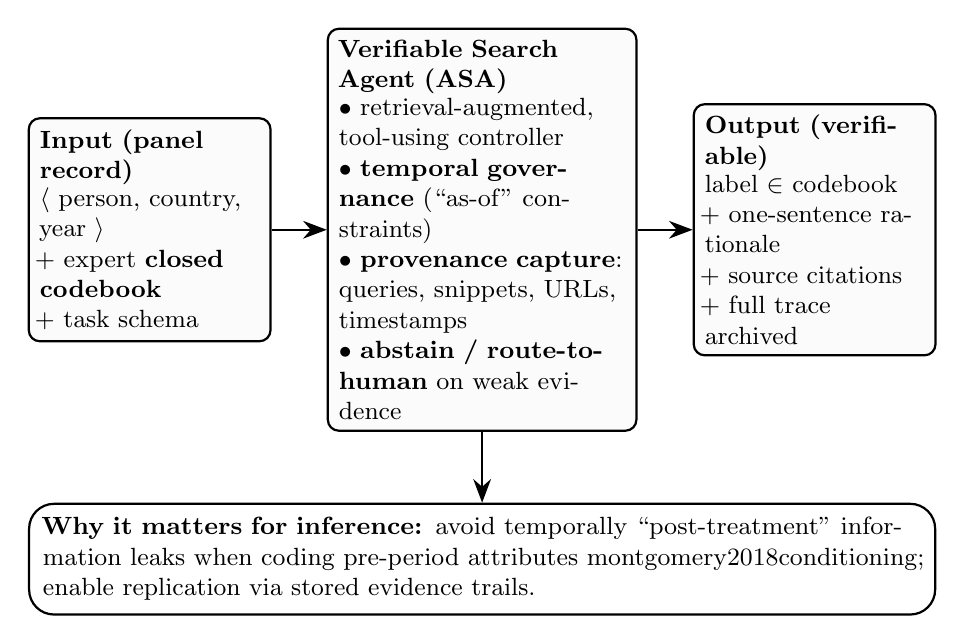
\begin{tikzpicture}[
    font=\small,
    node distance=9mm and 7mm,
    box/.style={rounded corners, draw=black, thick, fill=gray!3, inner sep=4pt, align=left},
    pill/.style={rounded corners=9pt, draw=black, thick, fill=white, inner sep=5pt, align=left},
    arr/.style={-{Stealth[length=3mm]}, thick},
  ]
    \node[box, text width=0.23\linewidth] (input) {
      \textbf{Input (panel record)}\\[-1pt]
      \(\langle\) person, country, year \(\rangle\)\\
      + expert \textbf{closed codebook}\\
      + task schema
    };

    \node[box, right=of input, text width=0.30\linewidth] (agent) {
      \textbf{Verifiable Search Agent (ASA)}\\[-1pt]
      \(\bullet\) retrieval-augmented, tool-using controller\\
      \(\bullet\) \textbf{temporal governance} (``as-of'' constraints)\\
      \(\bullet\) \textbf{provenance capture}: queries, snippets, URLs, timestamps\\
      \(\bullet\) \textbf{abstain / route-to-human} on weak evidence
    };

    \node[box, right=of agent, text width=0.23\linewidth] (output) {
      \textbf{Output (verifiable)}\\[-1pt]
      label \(\in\) codebook\\
      + one-sentence rationale\\
      + source citations\\
      + full trace archived
    };

    \draw[arr] (input) -- (agent);
    \draw[arr] (agent) -- (output);

    \node[pill, below=9mm of agent, text width=0.92\linewidth] (why) {
      \textbf{Why it matters for inference:} avoid temporally ``post-treatment'' information leaks when coding pre-period attributes \citep{montgomery2018conditioning}; enable replication via stored evidence trails.
    };
    \draw[arr] (agent.south) -- (why.north);
  \end{tikzpicture}%
  \caption{Visual abstract: the ASA treats web retrieval as a governed, auditable measurement process rather than an opaque chat interaction.}
  \label{fig:visual-abstract}
\end{figure}

\section{Motivation: why ``just use a search-enabled LLM'' is not enough}

Digital sources make it feasible to code political-elite attributes at scale, but research-grade datasets impose requirements that differ from interactive question answering.
In practice, a default workflow---``ask a search-enabled model for the answer''---tends to fail on three dimensions central to quantitative political science.

\paragraph{Auditability and replication.}
Elite attribute labels are \emph{measurements}. When the underlying retrieval context is not archived (queries, results, snippets, URLs, timestamps), a label is difficult to verify and cannot be re-audited when coders disagree or sources change.
This is especially problematic for downstream users who need to understand measurement error and may wish to apply alternative inclusion rules (e.g., discarding any label lacking a primary source).

\paragraph{Cross-national comparability.}
Many elite variables are \emph{categorical} and country-specific (e.g., party labels). ``Open-world'' generation invites label drift (synonyms, translations, rebrandings), undermining comparability across countries and years.
Closed codebooks supplied by domain experts are a natural remedy, but generic search-enabled chat systems do not typically enforce them.

\paragraph{Temporal leakage and post-treatment bias.}
Political elites switch parties, offices, and coalitions. If coding for year \(t\) uses sources written after \(t\) (e.g., biographies updated in 2025), the measurement can incorporate information that is itself caused by post-\(t\) outcomes.
This is a close analogue of conditioning on post-treatment variables in causal inference \citep{montgomery2018conditioning}: a label intended to reflect the pre-period state may be contaminated by later events, inducing bias in estimated relationships.
Temporal governance therefore belongs \emph{inside} the measurement protocol, not in ad hoc post-hoc cleaning.

\section{Methodology: a verifiable search agent}

We present a protocol---implemented as the \texttt{asa} software stack---that makes agent-based retrieval \emph{verifiable by construction}. The design has four core commitments:
\begin{enumerate}[leftmargin=*, itemsep=2pt]
\item \textbf{Closed-world decisions.} All predictions must lie in an expert-supplied codebook (e.g., the parties observed in a country-year panel).
\item \textbf{Evidence-first outputs.} Each label is paired with a terse rationale anchored to explicit source citations.
\item \textbf{Provenance preservation.} The system archives the full interaction trace: queries, tool responses, extracted snippets, URLs, and timestamps.
\item \textbf{Conservative abstention.} Under weak or conflicting evidence, the agent abstains (or routes to humans) rather than guessing.
\end{enumerate}

\subsection{Task formalization}

For each target record \(i\), the inputs are: a person name, a target country, an observation year \(t_i\), and a closed codebook \(\mathcal{C}_i\) supplied by expert coders.
The agent must return either (a) a label \(c \in \mathcal{C}_i\) with citations, or (b) an abstention.

\subsection{System design}

Operationally, the agent runs a short search session with read-only retrieval tools (e.g., Wikipedia and general web search), compiles candidate evidence, and emits a structured JSON result (label, one-sentence justification with citations, and a confidence category).
This design follows retrieval-augmented, tool-using agent patterns in the recent NLP literature \citep{yao2022react,lewis2020retrieval}.
A conservative post-processor then normalizes the label against the codebook: exact-match acceptance first, followed by a guarded fuzzy match for benign surface variation (punctuation, plurals, acronyms) using high similarity thresholds. This reduces typographic drift without introducing new classes.

\begin{figure}[htb]
  \centering
  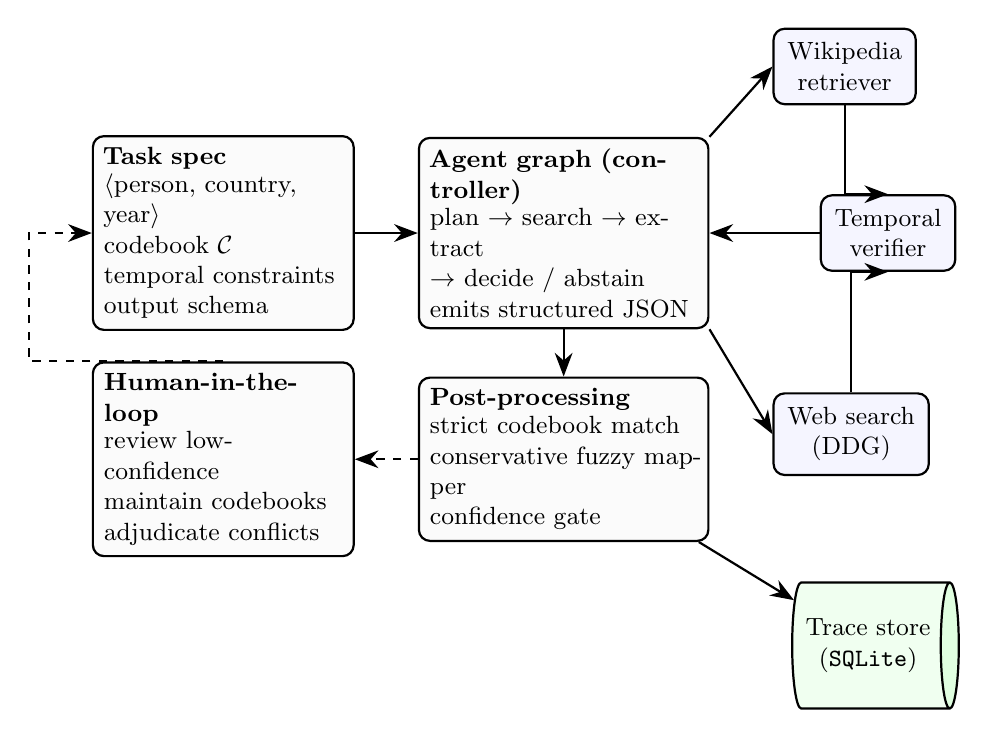
\begin{tikzpicture}[
    font=\small,
    node distance=6mm and 8mm,
    comp/.style={rounded corners, draw=black, thick, fill=gray!3, inner sep=4pt, align=left},
    tool/.style={rounded corners, draw=black, thick, fill=blue!4, inner sep=5pt, align=center},
    store/.style={cylinder, cylinder uses custom fill, cylinder body fill=green!6, cylinder end fill=green!12, draw=black, thick, aspect=0.25, minimum height=18mm, minimum width=16mm, align=center},
    arr/.style={-{Stealth[length=3mm]}, thick},
    loop/.style={-{Stealth[length=3mm]}, thick, dashed},
  ]
    \node[comp, text width=0.25\linewidth] (spec) {
      \textbf{Task spec}\\[-1pt]
      \(\langle\)person, country, year\(\rangle\)\\
      codebook \(\mathcal{C}\)\\
      temporal constraints\\
      output schema
    };

    \node[comp, right=of spec, text width=0.28\linewidth] (graph) {
      \textbf{Agent graph (controller)}\\[-1pt]
      plan \(\rightarrow\) search \(\rightarrow\) extract\\
      \(\rightarrow\) decide / abstain\\
      emits structured JSON
    };

    \node[tool, above right=4mm and 8mm of graph] (wiki) {Wikipedia\\retriever};
    \node[tool, below right=8mm and 8mm of graph] (web) {Web search\\(DDG)};
    \node[tool, right=14mm of graph] (time) {Temporal\\verifier};

    \node[comp, below=of graph, text width=0.28\linewidth] (post) {
      \textbf{Post-processing}\\[-1pt]
      strict codebook match\\
      conservative fuzzy mapper\\
      confidence gate
    };

    \node[store, below right=5mm and 12mm of post] (db) {Trace store\\(\texttt{SQLite})};

    \node[comp, left=of post, text width=0.25\linewidth] (human) {
      \textbf{Human-in-the-loop}\\[-1pt]
      review low-confidence\\
      maintain codebooks\\
      adjudicate conflicts
    };

    \draw[arr] (spec) -- (graph);
    \draw[arr] (graph) -- (post);
    \draw[arr] (post) -- (db);

    \draw[arr] (graph.north east) -- (wiki.west);
    \draw[arr] (graph.south east) -- (web.west);
    \draw[arr] (wiki.south) |- (time.north);
    \draw[arr] (web.north) |- (time.south);
    \draw[arr] (time.west) -- ([xshift=0mm]graph.east);

    \draw[loop] (post.west) -- (human.east);
    % Route this feedback loop outside the "Task spec" box (avoid striking through text).
    \draw[loop] (human.north) -| ([xshift=-8mm]spec.west) -- (spec.west);
  \end{tikzpicture}%
  \caption{Design visualization: a governed agent graph with temporal verification, conservative normalization, abstention, and an auditable trace store.}
  \label{fig:asa-design}
\end{figure}

\subsection{Temporal governance to prevent leakage}

The agent treats time as part of the measurement protocol. Each run is parameterized by an ``as-of'' rule: sources should be published before a cut date (e.g., \(t_i+1\) year) or within a target window around \(t_i\).
When feasible, the system extracts publication dates from retrieved pages and enforces the constraint strictly; otherwise it falls back to best-effort warnings and abstention rather than silently using potentially post-period material.
This guards against a common dataset-construction failure mode: coding pre-period attributes with post-period knowledge.

\subsection{Provenance preservation and storage}

All tool interactions and intermediate artifacts are persisted (including URLs and timestamps) to enable:
(i) verification of any individual label by following its citations, (ii) replication of aggregate statistics given the same trace store, and (iii) retrospective audits when codebooks change or new sources appear.
The storage design also supports alternative downstream rules (e.g., only keep labels supported by government sources).

\section{Case study: party affiliation inference at scale}

We evaluate ASA on a verifiable elite attribute: party affiliation. Using the subset of leader--records with expert codings, the agent attains an overall high-confidence accuracy of \LLMOverallAccHighpolparty{} across \LLMNumCountriespolparty{} countries (\(N=\) \LLMNumInstancespolparty{}), while expanding coverage by \LLMNumPredictionsGainedPercentpolparty{}\% (\LLMNumPredictionsGainedpolparty{} records) through conservative augmentation.
Low-confidence outputs are withheld by design, trading recall for precision; the mean share withheld is \LLMMeanLowConfpolparty{}.

\begin{figure}[htb]
  \centering
  \includegraphics[width=0.92\linewidth]{AgentHist.pdf}
  \caption{Agent performance in predicting party across countries with sufficient expert overlap. High-confidence predictions are evaluated against expert labels.}
  \label{fig:agent-performance}
\end{figure}

\begin{figure}[htb]
  \centering
  \includegraphics[width=0.60\linewidth]{AgentOverTime.pdf}
  \includegraphics[width=0.37\linewidth]{AgentRegionBox.pdf}
  \caption{Performance heterogeneity by time (left) and region (right).}
  \label{fig:agent-heterogeneity}
\end{figure}

% Required packages for the tables:
% \usepackage{booktabs}
% \usepackage{array}
% \usepackage{ragged2e}
% \usepackage{tabularx}
% \usepackage[table]{xcolor}
% \usepackage{hyperref}
% \usepackage{threeparttable}
%
% Recommended customizations (preamble):
% \definecolor{RowShade}{gray}{0.96}
% \newcolumntype{P}[1]{>{\RaggedRight\arraybackslash}p{#1}}
% \newcolumntype{C}[1]{>{\Centering\arraybackslash}p{#1}}
% \newcolumntype{Y}{>{\RaggedRight\arraybackslash}X}

\begin{table}[htbp]
\centering
\begingroup\setlength{\tabcolsep}{5pt}\renewcommand{\arraystretch}{1.18}
\begin{threeparttable}
\caption{Sample agent traces. Text content truncated for readability (and may contain typograical errors as present in native source). Links are clickable. Full traces contain many more sources.}
\label{tab:sample_compact}
\scriptsize
\begin{tabularx}{\linewidth}{@{}P{2.8cm}Y@{}}
\toprule
\textbf{Field} & \textbf{Content} \\
\midrule\rowcolor{RowShade}\multicolumn{2}{@{}l}{\textbf{Entry 1:} \textbf{Syleiman Abusaidovich Kerimov} — Russian Federation (1999)} \\
\addlinespace[0.25em]
\textbf{Country} & Russian Federation \\
\textbf{Year} & 1999 \\
\textbf{Person} & Syleiman Abusaidovich Kerimov \\
\textbf{Wikipedia} & Page: Ashot Egiazaryan Summary: Ashot Gevorkovich Egiazaryan (Russian: Ашот Геворкович Егиазарян; Armenian: Աշոտ Գեւորգովիչ Էկիազարյան; born... \\
\textbf{Search 1} & In the spring of 1998, Yeltsin dismissed Chernomyrdin as head of government and in1999Yeltsin's administration backed a newly formedparty,Un... \\
\textbf{URL 1} & \href{https://en.wikipedia.org/wiki/Our_Home_–_Russia https://en.wikipedia.org/wiki/Suleyman_Kerimov}{\footnotesize https://en.wikipedia.org/...} \\
\textbf{Search 2} & OURHOMEISRUSSIAPARTYOurHomeIsRussia(Nash Dom—Rossiya, or NDR) was a sociopolitical movement and a rulingpartyfrom 1996 to 1998. Source for i... \\
\textbf{URL 2} & \href{https://www.encyclopedia.com/history/encyclopedias-almanacs-transcripts-and-maps/our-home-russia-party https://tadviser.com/index.php/Person:Suleyman_Abusaidovich_Kerimov}{\footnotesize https://www.encyclopedia.com/...} \\
\addlinespace[0.35em]\cmidrule(lr){1-2}\addlinespace[0.15em]
\rowcolor{RowShade}\multicolumn{2}{@{}l}{\textbf{Entry 2:} \textbf{Jasminka Stanojevic} — Serbia (2018)} \\
\addlinespace[0.25em]
\textbf{Country} & Serbia \\
\textbf{Year} & 2018 \\
\textbf{Person} & Jasminka Stanojevic \\
\textbf{Wikipedia} & Page: Supreme Court (Serbia) Summary: The Supreme Court (Serbian: Врховни суд, romanized: Vrhovni sud) is the court of last resort in Serbia... \\
\textbf{Search 1} & This article lists political parties inSerbia, including parties that existed in the Kingdom ofSerbiabetween the early 1860s and 1918. A kol... \\
\textbf{URL 1} & \href{https://en.wikipedia.org/wiki/List_of_political_parties_in_Serbia https://www.kurir.rs/vesti/politika/2891361/22-godina-od-egzodusa-srba-u-oluji-ocajna-jasminka-stanojevic-deca-su-se-godinama-nadala-da-je-otac-ziv}{\footnotesize https://en.wikipedia.org/...} \\
\textbf{Search 2} & Imali su dve i četiri godine kad smo izbegli iz Knina. Kad bi neko pokucao na vrata, vikali bi: „Tata, tata". Tri godine nakon progona sazna... \\
\textbf{URL 2} & \href{https://www.kurir.rs/vesti/politika/2891361/22-godina-od-egzodusa-srba-u-oluji-ocajna-jasminka-stanojevic-deca-su-se-godinama-nadala-da-je-otac-ziv https://www.facebook.com/public/Jasminka-Stanojevic/}{\footnotesize https://www.kurir.rs/...} \\
\addlinespace[0.35em]\cmidrule(lr){1-2}\addlinespace[0.15em]
\rowcolor{RowShade}\multicolumn{2}{@{}l}{\textbf{Entry 3:} \textbf{Mihai STROE} — Romania (2011)} \\
\addlinespace[0.25em]
\textbf{Country} & Romania \\
\textbf{Year} & 2011 \\
\textbf{Person} & Mihai STROE \\
\textbf{Wikipedia} & Page: Adrian Stroe Summary: Adrian Stroe (born 24 October 1959), known as The Taxi Driver of Death, is a Romanian serial killer responsible ... \\
\textbf{Search 1} & Născut în Bucureşti şi cu origini în comuna argeşeană Morăreşti, fost medaliat cu aur la olimpiada internaţională de informatică,MihaiStroe(... \\
\textbf{URL 1} & \href{https://adevarul.ro/stiri-locale/pitesti/povestea-fascinanta-a-romanului-care-a-ajuns-1720222.html https://www.cdep.ro/pls/parlam/structura2015.mp?idm=286\&cam=2\&leg=2008\&pag=0 https://www.youtube.com/mihaistroetv}{\footnotesize https://adevarul.ro/...} \\
\textbf{Search 2} & MihaiSTROEParliamentary activity in legislature 2008-2012 DEPUTY Constituency no.38 TULCEA, uninominal college no.2 Membru al PDL, deputatul... \\
\textbf{URL 2} & \href{https://www.cdep.ro/pls/parlam/structura2015.mp?idm=286\&cam=2\&leg=2008\&idl=2 https://adevarul.ro/stiri-locale/tulcea/deputatul-democrat-liberal-mihai-stroe-nu-cred-1118196.html https://www.instagram.com/stroemihai/}{\footnotesize https://www.cdep.ro/...} \\
\addlinespace[0.35em]\cmidrule(lr){1-2}\addlinespace[0.15em]
\rowcolor{RowShade}\multicolumn{2}{@{}l}{\textbf{Entry 4:} \textbf{Matsie Angelina Motshekga} — South Africa (2018)} \\
\addlinespace[0.25em]
\textbf{Country} & South Africa \\
\textbf{Year} & 2018 \\
\textbf{Person} & Matsie Angelina Motshekga \\
\textbf{Wikipedia} & Page: Angie Motshekga Summary: Matsie Angelina "Angie" Motshekga (born 19 June 1955) is a South African politician and educator who is curre... \\
\textbf{Search 1} & MatsieAngelina"Angie"Motshekga(born 19 June 1955) is a SouthAfricanpolitician and educator who is currently serving as the Minister of Defen... \\
\textbf{URL 1} & \href{https://en.wikipedia.org/wiki/Angie_Motshekga}{\footnotesize https://en.wikipedia.org/wiki/Angie\_Motshekga} \\
\textbf{Search 2} & Motshekgawas elected thenationalpresident of theAfricanNationalCongressWomen's League (ANCWL) in 2008, defeating the League's secretary-gene... \\
\textbf{URL 2} & \href{https://www.sahistory.org.za/people/matsie-angelina-motshekga-angie-motshekga}{\footnotesize https://www.sahistory.org.za/people/matsie-angelina-motshekga-angie-motshekga} \\

\bottomrule
\end{tabularx}
\begin{tablenotes}
\footnotesize
\item 
\end{tablenotes}
\end{threeparttable}
\endgroup
\end{table}


\section{Discussion: design tradeoffs and practical guidance}

\paragraph{Cost and scaling.}
The methodology is built for high throughput: each record triggers a short, budgeted tool-usage episode and yields a structured output that can be scored, filtered, and aggregated without manual parsing.
Using smaller instruction-tuned models for orchestration, caching retrieval outputs, and routing only uncertain cases to humans yields substantial cost savings relative to fully manual coding or repeated interactive browsing.

\paragraph{What this approach does (and does not) guarantee.}
Provenance capture makes the \emph{evidence} for each label inspectable, but it does not magically eliminate ambiguity in the world.
The point of abstention is to keep ambiguity from silently becoming noise.
Similarly, temporal governance reduces leakage risk, but cannot fully recover historical truth when the web record is sparse.

\paragraph{When to use ASA.}
ASA is best suited to \emph{verifiable attributes} with authoritative sources (party membership, office holding, election outcomes) and stable codebooks.
For sensitive or non-verifiable attributes (e.g., ethnicity without self-identification), we recommend stricter abstention and explicit ethical review.

\section{Conclusion}

For political-elite research, the central question is not whether LLMs can answer factual questions, but whether they can be integrated into a \emph{measurement protocol} that is auditable, comparable, temporally well-defined, and cost-effective at scale.
The verifiable search agent methodology operationalizes these requirements through closed codebooks, evidence-first outputs, strict trace preservation, and conservative abstention.
This design turns retrieval-augmented agents into replicable instruments for dataset construction rather than opaque assistants.

\printbibliography

\end{document}
